%%%%%%%%%%%%%%%%%%%%%%%%%%%%%%%%%%%%%%
% LaTeX poster template
% Created by Nathaniel Johnston
% August 2009
% http://www.nathanieljohnston.com/index.php/2009/08/latex-poster-template/
%%%%%%%%%%%%%%%%%%%%%%%%%%%%%%%%%%%%%%

\documentclass[final]{beamer}
\usepackage[size=a0, orientation=portrait, scale=0.85]{beamerposter}
\usepackage{graphicx}			% allows us to import images
\usepackage{subfig}
%\setbeamertemplate{caption}[numbered]

%-----------------------------------------------------------
% Define the column width and poster size
% To set effective sepwid, onecolwid and twocolwid values, first choose how many columns you want and how much separation you want between columns
% The separation I chose is 0.024 and I want 4 columns
% Then set onecolwid to be (1-(4+1)*0.024)/4 = 0.22
% Set twocolwid to be 2*onecolwid + sepwid = 0.464
%-----------------------------------------------------------

\newlength{\sepwid}
\newlength{\onecolwid}
\newlength{\twocolwid}
\newlength{\threecolwid}
\setlength{\sepwid}{0.021739130434782608\paperwidth}
\setlength{\onecolwid}{0.30434782608695654\paperwidth}
\setlength{\twocolwid}{0.63043478260869568\paperwidth}
\setlength{\threecolwid}{0.95652173913043481\paperwidth}
\setlength{\topmargin}{-0.5in}
\usetheme{confposter}

%-----------------------------------------------------------
% Define colours (see beamerthemeconfposter.sty to change these colour definitions)
%-----------------------------------------------------------

\setbeamercolor{block title}{fg=ucdblue,bg=white}
\setbeamercolor{block body}{fg=black,bg=white}
\setbeamercolor{block alerted title}{fg=white,bg=ucdblue}
\setbeamercolor{block alerted body}{fg=black,bg=ucdblue!10}

%-----------------------------------------------------------
% User customizations
%-----------------------------------------------------------
% Reduce matrix size to fit in column
%http://tex.stackexchange.com/questions/43065/matrices-too-big-to-fit-the-width-of-a-page
\newcommand\scalemath[2]{\scalebox{#1}{\mbox{\ensuremath{\displaystyle #2}}}}

%-----------------------------------------------------------
% Name and authors of poster/paper/research
%-----------------------------------------------------------

\title{Identification of manual control employed during bicycling}

\author{Jason K. Moore, Mont Hubbard, and Ronald Hess}

\institute
{
\centering
\begin{tabular}{c}
Department of Mechanical and Aerospace Engineering, University of California, Davis\\
\end{tabular}
}
%-----------------------------------------------------------
% Start the poster itself
%-----------------------------------------------------------
% The \rmfamily command is used frequently throughout the poster to force a serif font to be used for the body text
% Serif font is better for small text, sans-serif font is better for headers (for readability reasons)
%-----------------------------------------------------------

\begin{document}
\frame{

\begin{center}
% Divide the frame into columns
\begin{columns}[t] % the [t] option aligns the column's content at the top

% Space column
\begin{column}{\sepwid}\end{column} % empty spacer column

% First column
\begin{column}{\onecolwid}

  \begin{block}{Introduction}
    \rmfamily{
      When balancing and directing a bicycle the human rider senses his or her
      motion and the environment and then actuates the body to cause the
      bicycle to travel in the desired direction. This requires both
      stabilization, as the bicycle-rider system is, in general, an unstable
      system, and path following. The most effective control input for
      controlling a bicycle under typical operation is to apply forces to cause
      the front frame to rotate about the steering axis. But riders are also
      capable of using other body motions to enable control of a bicycle. It is
      possible to predict the control actions of the rider using manual control
      theory but there have been few attempts to do so while controlling
      bicycles or motorcycles.

      We have collected a large set of time history data from an instrumented
      bicycle which includes the most important kinematic and kinetic variables
      to describe the bicycle-rider motion from three different riders on the
      same bicycle for a variety of speeds. Furthermore, the instrumented
      bicycle was designed so that the riders were not able to move their legs
      or torso relative to the rear frame of the bicycle, to ensure that the
      assumption of rider rigidity of the Whipple bicycle model was as close to
      valid as possible and to enforce a single control input from the rider.
      In the experiments we perturbed the bicycle-rider system with an
      externally applied lateral force and measured the rider's response.

      \begin{figure}[h]
        \begin{center}
          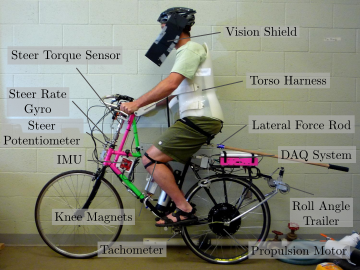
\includegraphics[width=6.5in]{figures/instrumented-bicycle.pdf}
          \caption{\rmfamily{(3)\quad Instrumented bicycle.}}
        \label{fig:Eig}
        \end{center}
      \end{figure}

      With the single-input multi-output data set in mind we formulate an 8th
      order grey box state space model \cite{Ljung1999} in the directly
      parameterized innovations form. The model is made up of the plant and the
      controller. Due to the poor predictive ability of the Whipple bicycle
      model we make use of a bicycle-rider system model identified from a
      larger superset of the data used here \cite{Moore2012}. We combine this
      model with a 2nd order model of the rider's neuromuscular system to form
      the plant. The controller structure is taken from \cite{Hess2012} which
      uses five gains nested in sequential feedback loops each simulating
      realistic sensory cues used by the rider.

      We then identify the unknown controller gains for each of the runs using
      the prediction error method, giving system models that predict the state
      trajectories with an average of $62 \pm 12$ percent of the variance
      accounted for (VAF) over all the identified runs. The resulting models
      are then analyzed and shown to hold well to the manual control theory
      presented in \cite{Hess2012}.
    } % rmfamily
  \end{block}

  \begin{block}{Continuous Control Model}
    \rmfamily{
      We bounded our controller identification to the controller design
      hypothesized in \cite{Hess2012}. The control structure was designed to
      meet these requirements:

      \begin{itemize}
        \item Roll stabilization is the primary task, with path following in
          the outer loops. The system should be stable in roll before closing
          the path following loops.
        \item The input to the bicycle and rider biomechanic model is steer
          torque. The neuromuscular mode of the closed system should have a
          natural frequency around 10 rad/s to match laboratory tracking tasks
          of a human operator.
        \item The system should be simple. In our case, only simple gains are
          needed to stabilize the system and close all the loops.
        \item We should see evidence of the crossover model in the open loop
          roll, heading, and lateral deviation loops.
      \end{itemize}

      The multi-loop model we use is constructed with a sequential loop closure
      technique that sets the model up to follow the dictates of the crossover
      model \cite{McRuer1967}. The three inner loops, \ref{fig:inner-loops},
      manage the roll stabilization task with steer angle $\delta$, roll rate
      $\dot{\phi}$, and roll angle $\phi$ feedback. The outer two loops,
      \ref{fig:outer-loops}, manage the path following with heading and lateral
      deviation feedback. We include a  simple second order model of the
      human's open-loop neuromuscular dynamics, $G_{nm}(s) =
      \frac{\omega^2}{s^2 + 2 \zeta \omega s + \omega^2}$,
      which produces a steer torque $T_\delta$ from the steer angle error. This
      model provides a parametric framework for the grey box identification of
      the controller gains and neuromuscular parameters.
    }

    \begin{figure}[h]
      \begin{center}
        \subfloat[]{\label{fig:inner-loops}\includegraphics[width=8in]{figures/inner-loops.pdf}}
        \\
        \subfloat[]{\label{fig:outer-loops}\includegraphics[width=8in]{figures/outer-loops.pdf}}
        \caption{\rmfamily{(4)\quad(a) Schematic of inner ``balance'' control
          loops. (b) Complete rider/vehicle feedback model.}}
      \end{center}
      \label{fig:Loops}
    \end{figure}

  \end{block}

\end{column}

% Spacer column
\begin{column}{\sepwid}\end{column} % empty spacer column

% Second column
\begin{column}{\onecolwid}

  \begin{block}{Experiments}
    \rmfamily{
      The analysis herein focuses on two maneuvers we call \emph{Heading
      Tracking} and \emph{Lateral Deviation Tracking}. During heading tracking
      the rider was instructed simply to balance the bicycle and keep a
      relatively constant heading while focusing their vision at a point in the
      distance. During lateral deviation tracking the rider focused on a
      straight line marked on the ground and attempted to keep the front wheel
      on this line. Both tasks were performed with random manually applied
      lateral perturbation forces, $F$, just below the seat, random in
      direction and time during the trials. Each maneuver was performed on both
      a 1 meter wide treadmill and an open gymnasium floor \cite{Moore2012}. We
      collected data from these two maneuvers for three subjects at speeds from
      1.5 m/s to 9.5 m/s for a total of 262 runs.
    }
  \end{block}

  \begin{block}{Identification}
    \rmfamily{
      We formulated two continuous grey box models, one for each maneuver. The
      heading tracking model did not include the lateral deviation feedback
      loop and the lateral deviation tracking model did. The bicycle model was
      found from a separate identification procedure \cite{Moore2012} which
      identified a fourth order model from a larger subset of the collected
      data. This identified portion of the plant ensured a realistic
      relationship between the steer torque input and the system outputs, as
      the first principles Whipple model was not sufficiently predictive.

      The state and input matrices of the closed loop system take this form:

      \begin{equation}
        \mathbf{A}
        =
        \left[
        \scalemath{0.8}{
        \begin{smallmatrix}
         0 & 0 & 1 & 0 & 0 & 0 & 0 & 0\\
         0 & 0 & 0 & 1 & 0 & 0 & 0 & 0\\
         a_{b\ddot{\phi}\phi} &
         a_{b\ddot{\phi}\delta} &
         a_{b\ddot{\phi}\dot{\phi}} &
         a_{b\ddot{\phi}\dot{\delta}} &
         0 & 0 & 0 & 0\\
         a_{b\ddot{\delta}\phi} &
         a_{b\ddot{\delta}\delta} &
         a_{b\ddot{\delta}\dot{\phi}} &
         a_{b\ddot{\delta}\dot{\delta}} &
         0 & 0 & 0 & 0\\
         0 & a_{b\dot{\psi}\delta} & 0 & a_{b\dot{\psi}\dot{\delta}} & 0 & 0 & 0 & 0\\
         0 & 0 & 0 & 0 & a_{b\dot{y}_p\psi} & 0 & 0 & 0 \\
         0 & 0 & 0 & 0 & 0 & 0 & 0 & 1 \\
         -\omega^2 k_{\delta} k_{\dot{\phi}} k_{\phi} &
         -\omega^2 k_{\delta} (1 + c_{b y_q \delta} k_{\dot{\phi}} k_{\phi} k_{\psi} k_{y_q}) &
         -\omega^2 k_{\delta} k_{\dot{\phi}} &
         0 &
         -\omega^2 k_{\delta} k_{\dot{\phi}} k_{\phi} k_{\psi} (1 + c_{b y_q \psi} k_{y_q}) &
         -\omega^2 k_{\delta} k_{\dot{\phi}} k_{\phi} k_{\psi} k_{y_q} &
         -\omega^2 &
         -2 \omega \zeta
        \end{smallmatrix}
        } % scalemath
        \right]
      \end{equation}

      \begin{equation}
        \mathbf{B}
        =
        \begin{bmatrix}
         0 & 0 \\
         0 & 0 \\
         b_{b\ddot{\phi}F} & 0 \\
         b_{b\ddot{\delta}F} & 0 \\
         0 & 0 \\
         0 & 0 \\
         0 & \omega^2 k_{\delta} k_{\dot{\phi}} k_{\phi} k_{\psi} k_{y_q}
        \end{bmatrix}
      \end{equation}

      Where the states are

      \begin{equation}
        x = \left[ \phi \quad \delta \quad \dot{\phi} \quad \dot{\delta}
        \quad \psi \quad y_p \quad T_\delta \quad \dot{T}_\delta \right]^T
      \end{equation}

      and the inputs are

      \begin{equation}
        u = \left[ F \quad y_{qc} \right]^T
      \end{equation}

      The only unknowns in the system are the controller gains and the
      neuromuscular model's natural frequency and damping terms, $\omega$,
      $\zeta$. The $a$ and $b$ entries are associated with the bicycle model
      and are pre-identified.

      We then discretized this continuous system with a zero order hold and
      formulate the directly parameterized innovations form \cite{Ljung1999} of
      the discrete linear system. The one step ahead prediction of the system
      outputs can be used to define a regressive cost function in which the
      error in the measured outputs and the model's outputs can be minimized
      with respect to the unknown parameters. Given a set of data the unknown
      parameters are identified using the prediction error method. We identify
      the unknown parameters for each of the 262 runs.

    } % rmfamily
  \end{block}

  \begin{block}{Results}
    \rmfamily{
      We identified the gains and neuromuscular frequency for each run with a
      62\% average self-validated VAF for all runs and outputs. The identified
      models predict the outputs around the input response very well and less
      so when there is no external perturbation due to the output error
      formulation of the model. Thus the models capture the linear portion of
      the human's control scheme, and leaves the remnant to output error.
    }

    \begin{figure}[h]
      \begin{center}
        \includegraphics[width=8in]{figures/rider-id-treadmill-run.pdf}
        \caption{\rmfamily{Simulation of an identified model derived from the
          inputs and outputs (SIMO) of one of rider C's treadmill runs \#288
          (4.23 m/s) validated against the data from run \#289 (4.22 m/s). The
          black line is the processed and filtered (low pass 15 Hz) measured
          data, the blue line is the simulation from the identified SIMO model
          and the green line is the identified SISO model.}}
      \label{fig:rider-id-treadmill-run}
      \end{center}
    \end{figure}
  \end{block}

\end{column}

% Spacer column
\begin{column}{\sepwid}\end{column} % empty spacer column

% The third column
\begin{column}{\onecolwid}

  \begin{block}{Results}
    \rmfamily{
      The identified gains for each run, Fig. \ref{fig:par-vs-speed-box-all},
      have a large spread, which is to be expected in a output error model and
      with three different human subjects. But there are some trends:

      \begin{itemize}
        \item The gains increase with speed with $k_\phi$and $k_{yq}$ having
          small slopes.
        \item The low speed runs have much more spread. This is probably due to
          the fact that the human remnant is relatively large at these speeds
          and the model attempts to fit the noise.
        \item The ~9 m/s runs have poorer data quality due to the treadmill
          interference in the measurement electronics, thus the spread is
          large.
        \item The neuromuscular frequency stays relatively constant just below
          30 rad/s, barring the higher variability in the low speed runs.
        \item The gains may be reasonably characterized with simple linear
          relationships.
      \end{itemize}
    }

    \begin{figure}[h]
      \begin{center}
        \includegraphics[width=6.5in]{figures/par-vs-speed-box-all.pdf}
        \caption{\rmfamily{Each of the five identified parameters as a function
          of speed. The parameter values are grouped into 0.5 m/s speed bins
          and box plots showing their distributions are given for each speed
          bin. The red line gives the median of the speed bin, the box bounds
          the quartiles, and the whisker is 1.5 times the inner quartile range.
          The width of the boxes are proportional to the square root of the
          number of runs in the bin. The green line gives the linear fit to the
          median values which are weighted with respect to the inverse of the
          standard deviation of each speed bin. The neuromuscular frequency is
          the best constant that fits the data.}}
      \label{fig:par-vs-speed-box-all}
      \end{center}
    \end{figure}

    \rmfamily{
      The identified models also exhibited similar frequency domain
      characteristics to the hypothesized models in \cite{Hess2012}. We see the
      typical human neuromuscular pole in the roll rate closed loop around 10
      rad/s in both the identified data and the first principles models from
      \cite{Hess2012}, Fig. \ref{fig:neuro-compare}.
    }

    \begin{figure}[h]
      \begin{center}

        \subfloat[]{\label{fig:all-phiDot_phiDotc-4}\includegraphics[width=5.25in]{figures/all-phiDot_phiDotc-4.png}}
        \subfloat[]{\label{fig:benchmarkSteerClosed}\includegraphics[width=5.25in]{figures/benchmarkSteerClosed.eps}}
        \caption{\rmfamily{(a) Frequency responses of the identified closed
          roll rate loop around 4 m/s. The grey lines plot the response of each
          individual run in the speed bin while the solid black line give the
          mean gain and phase bounded by the dotted black lines which indicate
          the one sigma standard deviation. (b) Frequency response of the first
          principle derived closed loop roll rate loop for the benchmark
          bicycle~\cite{Meijaard2007} at 5 m/s.}}
      \label{fig:neuro-compare}
      \end{center}
    \end{figure}

    \rmfamily{
      The outer three loops crossover in sequence as predicted \cite{Hess2012}
      but at frequencies that suggest slightly more aggressive control. The
      crossover frequencies are also relatively constant with respect to speed,
      as expected, Fig. \ref{fig:crossover-all}. Finally, the closed loop
      tracking response, Fig. \ref{fig:all-yQ_yQc-4} shows a stable system for
      all runs and the tracking performance is 1 to 1 out to a bandwidth of
      10 rad/s and the phase is low out to a bandwidth of 1 rad/s.
    }

    \begin{figure}[h]
      \begin{center}

        \subfloat[]{\label{fig:crossover-all}\includegraphics[width=4.5in]{figures/crossover-all.pdf}}
        \subfloat[]{\label{fig:all-yQ_yQc-4}\includegraphics[width=5.5in]{figures/all-yQ_yQc-4.png}}
        \caption{\rmfamily{(a) Median crossover frequencies in rad/s for the
          open outer loops for all runs at all speeds. (b) Frequency responses
          of the closed loop system lateral deviation tracking response around
          4 m/s. The grey lines plot the response of each individual run in the
          speed bin while the solid black lines give the mean gain and phase
          bounded by the dotted black lines which indicate one standard
          deviation.}}
      \label{fig:results}
      \end{center}
    \end{figure}
  \end{block}

  % References
  \begin{block}{References}
    \tiny{\rmfamily{
    \bibliographystyle{ieeetr}
    \bibliography{references}
    }}
  \end{block}

\end{column}

% Last spacer column
\begin{column}{\sepwid}\end{column} % empty spacer column

\end{columns}
\end{center}

} % frame
\end{document}
